% 第 4 章 Specifying Operating Conditions
\bichapter{指定工作条件}{Specifying Operating Conditions}
\label{chap:ocv}

工作条件包括芯片工作时的工艺、电压与温度参数。可以为 block 指定工作条件，工具在这些条件下分析并优化 block。

默认情况下，工具用片上变异（on-chip variation，OCV）模式做时序分析，以建模芯片上工作条件的变化。工具还支持高级片上变异（advanced on-chip variation，AOCV），作为提高时序分析精度的可选方法。

本章包括以下主题：
\begin{itemize}
  \item 指定工作条件
  \item 用工艺标签做 PVT 匹配
  \item 报告 PVT 信息
  \item 片上变异延迟分析
  \item 指定时序 derating 因子
  \item AOCV 简介
  \item 为 AOCV 分析做准备
  \item 施加 AOCV 数据
  \item 基于文件的 AOCV 数据
  \item 验证 AOCV 数据
  \item 参数化片上变异分析简介
  \item POCV 数据格式
  \item 执行参数化片上变异分析
  \item 时钟再汇聚悲观量消除简介
  \item 启用时钟再汇聚悲观量消除
  \item 报告时钟再汇聚悲观量消除的计算
\end{itemize}

\section{指定工作条件}
\subsection*{Specifying the Operating Conditions}

block 的工作条件包括芯片工作时所处的工艺、电压与温度。IC Compiler II 在所指定的条件下分析并优化 block。early 分析与 late 分析可以使用同一组或不同的工作条件。

指定工作条件有两种方法。

\begin{itemize}
  \item 分别指定下列参数：
  \begin{itemize}
    \item 用 \cmd{set\_process\_number} 指定工艺因子。默认同时作用于 early 与 late 分析。若只给其中一种分析指定数值，使用 \opt{-early} 或 \opt{-late}。
    \item 用 \cmd{set\_voltage} 指定电压。默认同时作用于 early 与 late。若 early 分析要用不同数值，使用 \opt{-min}。
    \item 用 \cmd{set\_temperature} 指定温度。默认同时作用于 early 与 late。若 early 分析要用不同数值，使用 \opt{-min}。
  \end{itemize}
        这些命令默认作用于当前 corner 上 block 内的全部对象。可用 \opt{-corners} 指定受影响的 corner，用 \opt{-object\_list} 指定受影响的对象。
  \item 用 \cmd{set\_operating\_conditions} 指定工作条件。所指定的工作条件：
  \begin{itemize}
    \item 同时作用于 early 与 late 分析。若只用于其中一种，使用 \opt{-min} 或 \opt{-max}。
    \item 只作用于当前 corner。对多 corner 多 mode 设计，必须为 block 中每个 corner 指定工作条件。
  \end{itemize}
\end{itemize}

参考库可以包含多组工作条件。用 \cmd{report\_lib} 列出某个库中可用的工作条件并查看其特征。

一般只使用一种方法为 block 指定工作条件。若必须两种都用，例如为多电压设计设置工作电压以覆盖 SDC 文件中的工作条件，先用 \cmd{set\_operating\_conditions}，再用单条命令覆盖具体数值。

\begin{seeAlsoBox}
\textit{IC Compiler II Library Preparation User Guide}
\end{seeAlsoBox}

\section{用工艺标签做 PVT 匹配}
\subsection*{Using Process Labels for PVT Matching}

参考库中的单元可以针对一种或多种工作条件做特性化。对 block 中的门级单元做时序分析时，若为 block 指定的工作条件与参考库中该单元的工作条件完全匹配，工具使用该数据；否则使用最接近的匹配。

\begin{noteBox}
若参考库含有 scaling group，scaling group 内的插值被视为精确匹配。
\end{noteBox}

可以用工艺标签（process label）引导工具从参考库中选择合适的时序模型。工艺标签在库准备期间加到参考库的特性化点上，例如：
\begin{lstlisting}
icc2_lm_shell> read_db -process_label fast fast_lib_0p95v125c.db
\end{lstlisting}

要引导 IC Compiler II 对某个 corner 使用指定的特性化点，用 \cmd{set\_process\_label} 为该 corner 指定工艺标签：
\begin{lstlisting}
icc2_shell> create_corner c_fast
icc2_shell> set_process_label -corners c_fast fast
\end{lstlisting}

\section{报告 PVT 信息}
\subsection*{Reporting PVT Information}

用 \cmd{report\_pvt} 报告 PVT 信息，包括为 corner 指定的工作条件与 block 中所用单元时序视图之间的不匹配。报告包含所指定的 PVT 设置，以及找不到精确匹配时所实际使用的设置。

除 \cmd{report\_pvt} 外，还可以通过查询表~\ref{tab:pvt-attr} 中的时序属性，取得当前 block 所用的 PVT 值。

\begin{table}[htbp]
\centering
\caption{工作条件属性}
\label{tab:pvt-attr}
\small
\begin{tabularx}{\textwidth}{@{}l *{3}{>{\raggedright\arraybackslash}X}@{}}
\toprule
设置 & 指定值 & 解析值 & 不匹配计数 \\
\midrule
工艺标签 &
\cmd{process\_label\_early}\newline
\cmd{process\_label\_late} &
\cmd{effective\_process\_label\_early}\newline
\cmd{effective\_process\_label\_late} &
\cmd{process\_label\_mismatches} \\
工艺数值 &
\cmd{process\_number\_early}\newline
\cmd{process\_number\_late} &
\cmd{effective\_process\_number\_early}\newline
\cmd{effective\_process\_number\_late} &
\cmd{process\_number\_mismatches} \\
电压 &
\cmd{voltage\_early}\newline
\cmd{voltage\_late} &
\cmd{effective\_voltage\_early}\newline
\cmd{effective\_voltage\_late} &
\cmd{voltage\_mismatches} \\
温度 &
\cmd{temperature\_early}\newline
\cmd{temperature\_late} &
\cmd{effective\_temperature\_early}\newline
\cmd{effective\_temperature\_late} &
\cmd{temperature\_mismatches} \\
\bottomrule
\end{tabularx}
\end{table}

\section{片上变异延迟分析}
\subsection*{On-Chip Variation Delay Analysis}

时序分析期间，工具使用 OCV 模式。该模式同时把最小延迟与最大延迟加到不同路径上，从而做偏保守的时序分析。

对 setup 检查，工具对 launch 时钟路径与数据路径使用最大延迟，对 capture 时钟路径使用最小延迟，如图~\ref{fig:ocv-setup}。

\begin{figure}[htbp]
  \centering
  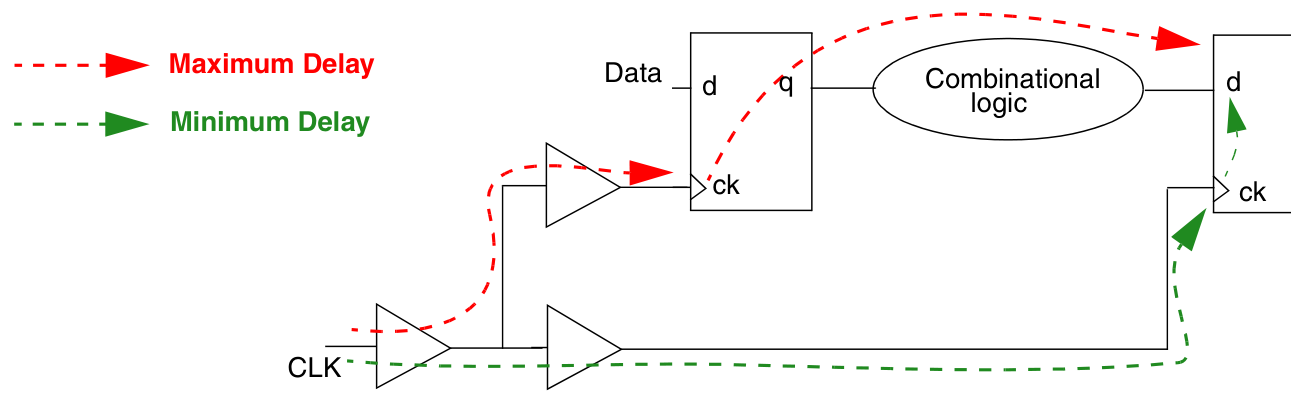
\includegraphics[width=0.88\textwidth]{fig-4-1.png}
  \caption{setup 分析中的片上变异}
  \label{fig:ocv-setup}
\end{figure}

对 hold 检查，工具对 launch 时钟路径与数据路径使用最小延迟，对 capture 时钟路径使用最大延迟，如图~\ref{fig:ocv-hold}。

\begin{figure}[htbp]
  \centering
  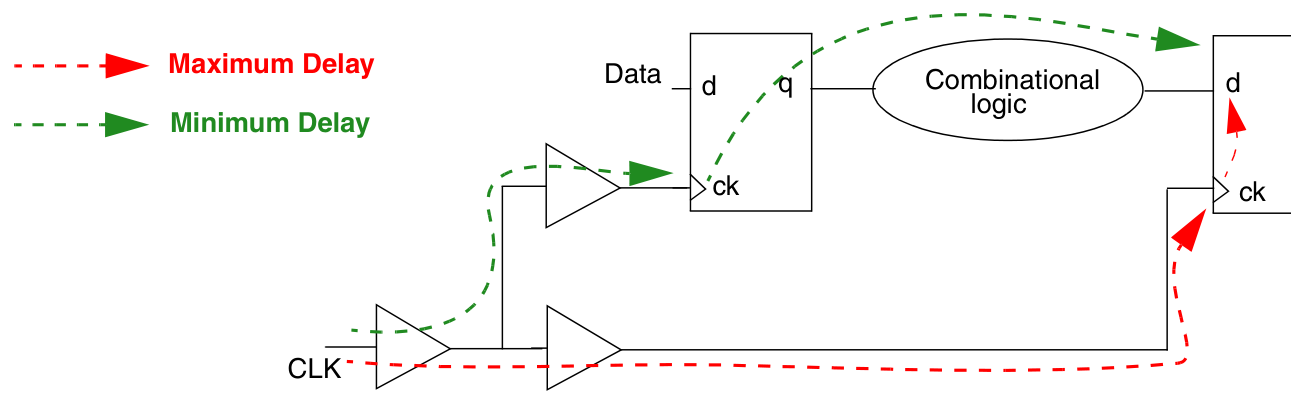
\includegraphics[width=0.88\textwidth]{fig-4-2.png}
  \caption{hold 分析中的片上变异}
  \label{fig:ocv-hold}
\end{figure}

表~\ref{tab:setup-hold-params} 给出 setup 检查与 hold 分析所用的时钟到达时间、延迟、工作条件与 derating。

\begin{table}[htbp]
\centering
\caption{setup 与 hold 分析所用的时序参数}
\label{tab:setup-hold-params}
\begin{tabularx}{\textwidth}{@{}l X X X@{}}
\toprule
分析类型 & Launch 时钟路径 & 数据路径 & Capture 时钟路径 \\
\midrule
Setup &
Late 时钟，时钟路径最大延迟，late derating，最坏情况工作条件 &
最大延迟，late derating，最大工作条件 &
Early 时钟，时钟路径最小延迟，early derating，最小工作条件 \\
Hold &
Early 时钟，时钟路径最小延迟，early derating，最好情况工作条件 &
最小延迟，early derating，最小工作条件 &
Late 时钟，时钟路径最大延迟，late derating，最大工作条件 \\
\bottomrule
\end{tabularx}
\end{table}

时序分析期间，工具同时考虑下列设计参数所指定的最小值与最大值：输入与输出外部延迟、端口线负载模型、端口扇出数、网线电容、网线电阻、网线线负载模型、时钟 latency、时钟转换时间，以及输入端口的驱动单元。

\section{指定时序 derating 因子}
\subsection*{Specifying the Timing Derating Factors}

时序 derating 因子通过调整 block 中各时序弧的计算延迟，建模工作条件变化的影响。默认 derating 因子为 1.0，工具不调整计算得到的延迟。

用 \cmd{set\_timing\_derate} 设置 derating 因子，并指定：
\begin{itemize}
  \item derating 因子本身。
  \item 用 \opt{-early} 或 \opt{-late} 说明该因子用于 early 还是 late 延迟。
\end{itemize}

还可以把 derating 因子施加到：
\begin{itemize}
  \item 指定的叶级实例、层次实例或库单元。默认作用于当前 block。
  \item 只用 \opt{-rise} 或 \opt{-fall} 作用于上升或下降延迟。默认同时作用于两者。
  \item 只用 \opt{-clock} 或 \opt{-data} 作用于时钟路径或数据路径。默认同时作用于两者。
  \item 用 \opt{-net\_delay}、\opt{-cell\_delay} 或 \opt{-cell\_check} 作用于网线延迟、单元延迟或单元时序检查。默认三者都作用。用 \cmd{set\_timing\_derate -net\_delay} 为网线延迟指定 derating 时，同时作用于网线延迟的动态分量与静态分量。可用 \opt{-dynamic} 与 \opt{-static} 为两个分量指定不同因子。
  \item 用 \opt{-corners} 作用于指定 corner。默认作用于当前 corner。
\end{itemize}

要用增量修改已有 timing derate，使用 \opt{-increment}。该增量加到已有 derating 因子上。

下例把当前 corner 的全部最小延迟减小 10\%，全部最大延迟增大 20\%：
\begin{lstlisting}
icc2_shell> set_timing_derate -early 0.9 -late 1.2
\end{lstlisting}

用 \cmd{report\_timing\_derate} 报告 derating 因子。默认报告全部 corner；用 \opt{-corners} 报告指定 corner。

用 \cmd{reset\_timing\_derate} 把 derating 因子复位为 1.0。默认复位当前 corner 上当前 block 及其全部单元实例的因子。用 \opt{-corners} 复位指定 corner，或指定对象以复位这些对象上的因子。

\section{AOCV 简介}
\subsection*{Introduction to AOCV}

高级片上变异（AOCV）是一种可选方法：按路径深度或物理距离跨度，对不同路径使用不同的 derating 因子，从而提高精度。逻辑级数更多或物理距离更长的路径，总变异往往更小，因为门与门之间的随机变异趋于相互抵消。因此 AOCV 对短路径使用较高的 derating，对长路径使用较低的 derating。

这种方法比传统 OCV 更不悲观。传统 OCV 依赖不考虑路径具体度量的常数 derating。精度提高会同时影响时序报告与设计优化。

IC Compiler II 的 AOCV 流程包括以下高层步骤：
\begin{enumerate}
  \item 按「为 AOCV 分析做准备」设置 AOCV 分析。
  \item 按「施加 AOCV 数据」施加 AOCV 数据。
  \item 按「验证 AOCV 数据」验证 AOCV 数据。
  \item 使用 AOCV 数据做时序分析与优化。
\end{enumerate}

\section{为 AOCV 分析做准备}
\subsection*{Setting Up for AOCV Analysis}

把应用选项 \appopt{time.aocvm\_enable\_analysis} 设为 \cmd{true} 以启用 AOCV 分析。

还可以用下列应用选项改变默认行为：
\begin{itemize}
  \item 把 \appopt{time.aocvm\_enable\_clock\_network\_only} 设为 \cmd{true}，使 AOCV 只分析时钟网络。默认同时分析时钟网络与数据网络。
  \item 用 \appopt{time.aocvm\_analysis\_mode} 改变 AOCV 分析中路径深度的计算方式，有三种设置：
  \begin{itemize}
    \item \cmd{separate\_launch\_capture\_depth}：默认。同时使用时钟与数据网络对象，并为 capture 路径与 launch 路径分别计算深度。
    \item \cmd{combined\_launch\_capture\_depth}：同时使用时钟与数据网络对象，把 capture 与 launch 合在一起计算整条路径的深度。
    \item \cmd{separate\_data\_and\_clock\_metrics}：为时钟路径与数据路径分别计算深度。
  \end{itemize}
  \item 把 \appopt{time.ocvm\_enable\_distance\_analysis} 设为 \cmd{true}，在门计数之外再考虑物理距离。默认不考虑路径的物理距离。
  \item 把 \appopt{time.aocvm\_enable\_single\_path\_metrics} 设为 \cmd{true}，只用单元距离与深度度量来导出单元和网线的 AOCV derating。
  \item 把 \appopt{time.ocvm\_precedence\_compatibility} 设为 \cmd{true}，当存在 AOCV derating 时忽略由 \cmd{set\_timing\_derate} 指定的 OCV derating。默认同时考虑 OCV 与 AOCV，优先级从高到低为：
  \begin{enumerate}
    \item 叶单元上的 OCV derate
    \item 库单元上的 AOCV derate
    \item 库单元上的 OCV derate
    \item 层次单元上的 AOCV derate
    \item 层次单元上的 OCV derate
    \item 设计上的 AOCV derate
    \item 设计上的 OCV derate
  \end{enumerate}
\end{itemize}

\section{施加 AOCV 数据}
\subsection*{Applying AOCV Data}

AOCV 时序分析期间，工具根据路径中相继的门数（路径深度），以及可选的路径物理距离跨度，从 AOCV 数据导出 derating 值。

提供 AOCV 数据有两种方法：
\begin{itemize}
  \item 使用逻辑库（\cmd{.db}）中基于库的 AOCV 数据。
  \item 使用基于文件的 AOCV 数据，用 \cmd{read\_ocvm} 读入。
\end{itemize}

用 \opt{-corners} 为指定 corner 施加 AOCV 数据。基于库与基于文件的 AOCV 数据都可以由 Synopsys SiliconSmart 特性化工具生成。细节见 SolvNet 上的 \textit{SiliconSmart ACE User Guide}。

可以同时使用基于库与基于文件的 AOCV derating。冲突时优先级从高到低为：
\begin{enumerate}
  \item 库单元上基于文件的 AOCV derate
  \item 层次单元上基于文件的 AOCV derate
  \item 设计上基于文件的 AOCV derate
  \item 库单元或库上基于库的 AOCV derate
\end{enumerate}

还可以指定：
\begin{itemize}
  \item 用 \cmd{set\_timing\_derate -aocvm\_guardband} 为 AOCV derating 因子设置保护带。下例为 early 与 late 延迟指定 5\% 的保护带：
\begin{lstlisting}
icc2_shell> set_timing_derate -aocvm_guardband -early 0.95
icc2_shell> set_timing_derate -aocvm_guardband -late 1.05
\end{lstlisting}
  \item 用 \cmd{set\_aocvm\_coefficient} 在库单元或单元实例级设置深度调整系数。计算时序路径总深度（逻辑级数）时，工具默认把每个单元的深度计为 1。该命令可以增大或减小某个库单元的深度。下例把库单元 \cmd{MGX16} 的深度增至 1.5：
\begin{lstlisting}
icc2_shell> set_aocvm_coefficient 1.5 [get_lib_cells lib_fast/MGX16]
\end{lstlisting}
\end{itemize}

用 \cmd{remove\_ocvm} 从设计对象上去掉部分或全部 AOCV derating 值。

\section{基于文件的 AOCV 数据}
\subsection*{File-Based AOCV Data}

AOCV 数据文件把单元、库单元或网线的 derating 值指定为路径深度的函数，可选地也是路径所跨越物理距离的函数。IC Compiler II 接受 PrimeTime 中 \cmd{write\_binary\_aocvm} 产生的二进制与压缩数据文件。

表~\ref{tab:aocv-fmt} 给出 AOCV 文件格式的语法。

\begin{table}[htbp]
\centering
\caption{AOCV 文件格式语法}
\label{tab:aocv-fmt}
\begin{tabularx}{\textwidth}{@{}l X@{}}
\toprule
字段 & 说明 \\
\midrule
\cmd{version} & AOCV 版本号 \\
\cmd{object\_type} & \cmd{design | cell | lib\_cell} \\
\cmd{rf\_type} & \cmd{rise | fall | rise fall} \\
\cmd{delay\_type} & \cmd{cell | net | cell net} \\
\cmd{derate\_type} & \cmd{early | late} \\
\cmd{path\_type} & \cmd{clock | data | clock data} \\
\cmd{object\_spec} & 字符串 \\
\cmd{depth} & 一组 $M$ 个浮点数，$M$ 可以为 0 \\
\cmd{distance} & 一组 $N$ 个浮点数，$N$ 可以为 0。只有 \appopt{time.ocvm\_enable\_distance\_analysis} 为 \cmd{true} 时才使用距离值 \\
\cmd{table} & 一组 $N \times M$ 个浮点数。特殊情况：$N=0$ 时表的大小为 $M$；$M=0$ 时表的大小为 $N$；两者都为 0 时表的大小为 1。未定义的点用线性插值。工具不外推到表中最低值或最高值之外 \\
\bottomrule
\end{tabularx}
\end{table}

\cmd{object\_spec} 指定对象名。还可以使用按对象属性求值的表达式，类似于在创建 collection 的命令中使用 Tcl 的 \cmd{regexp}。\cmd{patterns} 字段可以使用相关 collection 命令的任意选项。例如 \cmd{object\_type} 为 \cmd{lib\_cell} 时，可以使用 \cmd{get\_lib\_cells} 的任意参数。

在文件任意位置加注释时，使用双斜杠（\cmd{//}）。

下例为整个设计中的时钟网线设置 early AOCV 表：
\begin{lstlisting}
version             1.0
object_type:        design
rf_type:            rise fall
delay_type:         cell net
derate_type:        early
path_type:          clock
object_spec:        top
depth:              0 1 2 3
distance:           100 200
table:              0.87 0.93 0.95 0.96 \
                    0.83 0.85 0.87 0.90
\end{lstlisting}

下例为工作条件电压为 1.2~V 的全部层次单元、时钟路径设置 late AOCV 表：
\begin{lstlisting}
version             1.0
object_type:        cell
rf_type:            rise
delay_type:         cell
derate_type:        late
path_type:          clock
object_spec:        * -filter (voltage_max==1.2 && is_hierarchical==true)
depth:              1  2  3
distance:           100  1000
table:              1.21  1.11  1.09 \
                    1.23  1.16  1.14
\end{lstlisting}

\section{验证 AOCV 数据}
\subsection*{Verifying AOCV Data}

用 \cmd{report\_ocvm} 查看 AOCV derate 表。可以查看标注了 early、late、rise、fall、cell 或 net derate 表的设计对象，也可以用该命令判断哪些单元和网线已标注或尚未标注 AOCV 信息。

例如，取得单元 \cmd{U57} 从引脚 A 到引脚 Z 的时序弧上的 AOCV derate 数据：
\begin{lstlisting}
icc2_shell> report_ocvm -type ocvm \
    [get_timing_arcs -from U57/I -to U57/Z]
\end{lstlisting}

\section{参数化片上变异分析简介}
\subsection*{Introduction to Parametric On-Chip Variation Analysis}

参数化片上变异（parametric on-chip variation，POCV）分析是一种可选的时序分析模式，用统计方法建模片上变异。在该模式下，工具把到达时间、要求时间与 slack 计算为统计分布，而不是固定的最小与最大值。时序结果更不悲观，为时序优化提供更好的依据。

POCV 时序分析不为每条时序弧指定绝对的最小与最大延迟，而是把延迟表示为高斯（正态）分布 $P$ 的函数：
\[
\mathrm{delay} = \mathrm{nominal\_delay} + \sigma \cdot P
= \mathrm{nominal\_delay} + (C \cdot \mathrm{nominal\_delay}) \cdot P
\]

工具从 \cmd{.db} 库取得延迟变异 $\sigma$（若库中有），或由 POCV 数据文件中提供的系数 $C$ 计算，其中 $\sigma = C \cdot \mathrm{nominal\_delay}$。

图~\ref{fig:pocv} 把传统 min-max 延迟与 POCV 统计延迟作图形比较。

\begin{figure}[htbp]
  \centering
  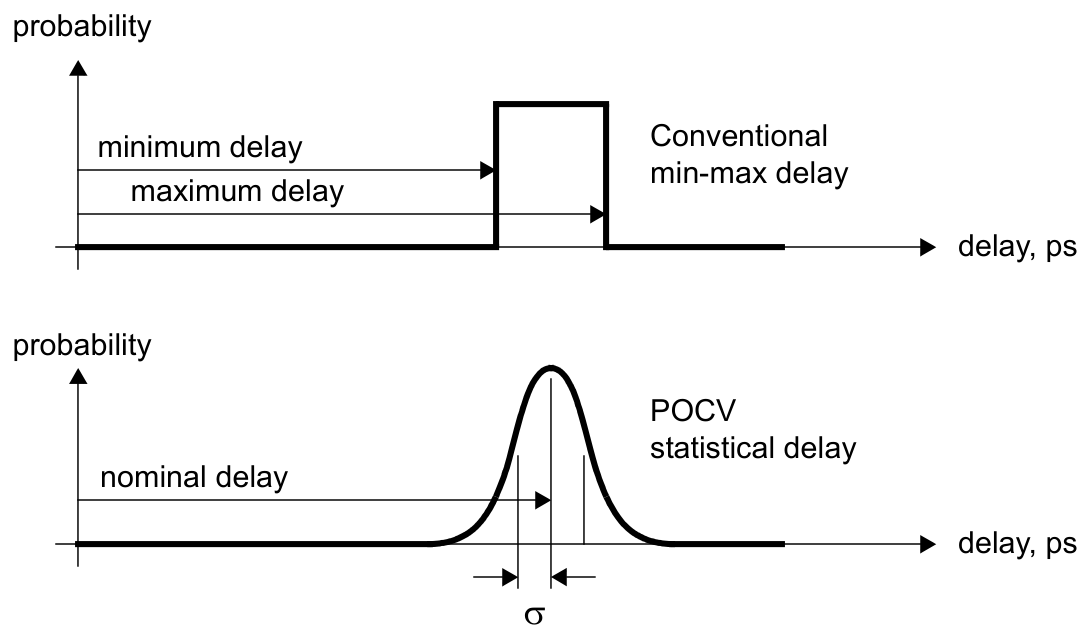
\includegraphics[width=0.78\textwidth]{fig-4-3.png}
  \caption{min-max 延迟与 POCV 统计延迟的比较}
  \label{fig:pocv}
\end{figure}

两种延迟变异的差别：
\begin{itemize}
  \item min-max 延迟为时序弧指定绝对最小与最大延迟。实际延迟在这两个极端之间任意位置出现的概率相等，超出这两个极端的概率为零。
  \item POCV 统计模型指定标称延迟与变异 $\sigma$。延迟在标称值处出现的概率最高，离标称值越远概率越小。实际延迟落在标称延迟 $3\sigma$ 范围内的概率为 99.7\%。
\end{itemize}

工具确定每条时序弧的延迟分布之后，沿时序路径做统计传播，把每个到达时间、要求时间与 slack 计算为总标称值加上累积变异。

计算路径累积延迟时，工具把每一级的延迟分布做统计合并。这比简单地把每一级的最坏情况值相加更准确。得到的延迟与 slack 比简单的 min-max 相加更现实、更不悲观。

默认情况下，\cmd{report\_timing} 报告的最终 slack 是比标称 slack 低三个标准差（$3\sigma$）的 slack：
\[
\mathrm{reported\_slack} = \mathrm{nominal\_slack} - 3\sigma
\]

可以把 sigma 乘数从 3.0 改大或改小，以收紧或放宽时序约束。

\section{POCV 数据格式}
\subsection*{POCV Data Formats}

执行 POCV 时序分析时，IC Compiler II 需要每条时序弧的变异 $\sigma$。提供该信息有两种方式。

\begin{itemize}
  \item \textbf{基于库的 POCV 数据}\\
        工具支持 Liberty Variation Format（LVF）中、基于 \cmd{.db} 库的 POCV 变异数据，覆盖延迟、转换时间与约束弧。
  \begin{itemize}
    \item 对延迟弧，每个 LVF 表项给出输入 slew 与输出负载某一组合下的延迟变异 $\sigma$。
    \item 对转换时间弧，每个 LVF 表项给出输入 slew 与输出负载某一组合下的转换时间变异 $\sigma$。
    \item 对约束弧，每个 LVF 表项给出被约束引脚与相关引脚转换时间某一组合下的约束变异 $\sigma$。
  \end{itemize}
\end{itemize}

\begin{noteBox}
若库中含有 LVF 表，请确认 IC Compiler II 设计库是用 K-2015.06-SP1 或更新版本的 IC Compiler II Library Manager 创建的。LVF 信息包含在设计库中，并在进入 IC Compiler II 会话时自动读入。
\end{noteBox}

\begin{itemize}
  \item \textbf{基于文件的 POCV 数据}\\
        用 \cmd{read\_ocvm} 为指定 corner 读入纯文本系数数据文件。系数文件含延迟变异数据，但不支持转换时间或约束变异数据。文件为文本中指定的每个库单元、层次单元或设计施加单一系数 $C$。延迟变异按 $\sigma = C \cdot \mathrm{nominal\_delay}$ 计算。一个单元的全部时序弧共用同一个系数 $C$，与输入 slew 和输出负载无关。
\end{itemize}

基于库与基于文件的 POCV 数据都可以由 SiliconSmart 生成。细节见 SolvNet 上的 \textit{SiliconSmart ACE User Guide}。

\subsection{基于文件的 POCV 数据}
\subsubsection*{File-Based POCV Data}

POCV 数据文件为设计、设计中的层次单元或设计所用的库单元指定延迟变异系数 $C$。工具接受 PrimeTime 中 \cmd{write\_binary\_aocvm} 产生的二进制与压缩数据文件。转换时间与约束变异必须使用基于 LVF 库的数据。POCV 分析始终同时作用于数据路径与时钟路径。

表~\ref{tab:pocv-fmt} 给出 POCV 数据文件的语法。

\begin{table}[htbp]
\centering
\caption{POCV 数据文件语法}
\label{tab:pocv-fmt}
\begin{tabularx}{\textwidth}{@{}l X@{}}
\toprule
字段 & 说明 \\
\midrule
\cmd{version} & 4.0（片上变异数据文件版本号，必须为 4.0 或更高） \\
\cmd{ocvm\_type} & \cmd{pocv}（参数化片上变异） \\
\cmd{object\_type} & \cmd{design | cell | lib\_cell} \\
\cmd{rf\_type} & \cmd{rise | fall | rise fall} \\
\cmd{delay\_type} & \cmd{cell | net | cell net} \\
\cmd{derate\_type} & \cmd{early | late} \\
\cmd{path\_type} & \cmd{clock | data | clock data} \\
\cmd{object\_spec} & 标注了 POCV 系数的对象名 \\
\cmd{coefficient} & 变异系数 \\
\bottomrule
\end{tabularx}
\end{table}

下例为库单元 \cmd{lib28/invx2} 的下降转换设置 POCV 系数：
\begin{lstlisting}
version:      4.0
ocvm_type:    pocvm
object_type:  lib_cell
rf_type rise: fall
delay_type :  cell
derate_type:  early
object_spec:  lib28/invx2
coefficient:  0.05
\end{lstlisting}

\cmd{object\_spec} 指定对象名，用法与 AOCV 文件相同：可按对象属性求值，并使用相关 collection 命令的选项。注释使用 \cmd{//}。

下例为整个设计的 early 延迟设置 POCV 系数：
\begin{lstlisting}
version:      4.0
ovcm_type:    pocv
object_type:  design
rf_type:      rise fall
delay_type:   cell net
derate_type:  early
object_spec:         // Leave object_spec blank if object_type is design
coefficient:  0.05
\end{lstlisting}

下例为工作条件电压为 1.2~V 的全部层次单元的 late 延迟设置 POCV 系数：
\begin{lstlisting}
version       4.0
ovcm_type:    pocv
object_type:  cell
rf_type:      rise
delay_type:   cell
derate_type:  late
object_spec:  * -filter (voltage_max==1.2 && is_hierarchical==true)
coefficient:  0.07
\end{lstlisting}

\subsection{文件 POCV 数据与库 POCV 数据的优先级}
\subsubsection*{Precedence of File- and Library-POCV Data}

可以同时使用基于文件与基于库的 POCV 数据。默认按下列优先级解决冲突，从高到低：
\begin{enumerate}
  \item 库单元上基于文件的 POCV 系数
  \item 层次单元上基于文件的 POCV 系数
  \item 设计上基于文件的 POCV 系数
  \item 库单元或库上基于库的 POCV LVF 数据
\end{enumerate}

用应用选项 \appopt{time.pocvm\_precedence} 改变默认优先级。默认值为 \cmd{file}。

\begin{itemize}
  \item 设为 \cmd{library} 时，优先级为：库单元或库上的 LVF 数据；库单元上的文件系数；层次单元上的文件系数；设计上的文件系数。
  \item 设为 \cmd{lib\_cell\_in\_file} 时，优先级为：库单元上的文件系数；库单元或库上的 LVF 数据；层次单元上的文件系数；设计上的文件系数。
\end{itemize}

\section{执行参数化片上变异分析}
\subsection*{Performing Parametric On-Chip Variation Analysis}

工具支持在时序分析与优化中做 POCV 分析。它需要 Liberty Variation Format（LVF）中基于文件或基于库的 POCV 数据，并支持延迟、转换时间与约束 LVF 表。POCV 分析也可以配合基于距离的 derate 表进行。

若库中含有 LVF 表，设计库须用 K-2015.06-SP1 或更新的 Library Manager 创建。LVF 信息会自动读入会话。

执行 POCV 分析的步骤：
\begin{enumerate}
  \item 为 block 定义全部 mode、corner 与 scenario。
  \item 用应用选项 \appopt{time.pocvm\_enable\_analysis} 启用 POCV 分析。
\begin{lstlisting}
icc2_shell> set_app_options -name time.pocvm_enable_analysis \
    -value true
\end{lstlisting}
  \item （可选）改变 POCV 分析中由统计参数计算最坏情况值所用的标准差（$\sigma$）个数：
  \begin{itemize}
    \item 改变整个 block 的值：使用 \appopt{time.pocvm\_corner\_sigma}。
    \item 改变指定 corner 的值：使用 \cmd{set\_pocvm\_corner\_sigma}。
  \end{itemize}
        默认时序分析使用相对均值 3 个标准差（$3\sigma$）处的值。增大标准差个数会收紧时序要求。
        下例把当前 block 的标准差个数改为 3.5，把名为 \cmd{corner1} 的 corner 改为 4：
\begin{lstlisting}
icc2_shell> set_app_options -name time.pocvm_corner_sigma \
    -value 3.5 -block [current_block]
icc2_shell> set_pocvm_corner_sigma -corners corner1 4.0
\end{lstlisting}
\begin{noteBox}
若先用 \cmd{set\_pocvm\_corner\_sigma} 施加 corner 专用值，再用 \appopt{time.pocvm\_corner\_sigma} 施加 block 专用值，后一次的 block 专用值会覆盖先前的 corner 专用值。
\end{noteBox}
  \item （可选）若 LVF 库含有 slew 变异数据，用 \appopt{time.enable\_slew\_variation} 在 POCV 分析中启用 slew 变异。
\begin{lstlisting}
icc2_shell> set_app_options -name time.enable_slew_variation -value true
\end{lstlisting}
  \item （可选）若 LVF 库含有约束变异数据，用 \appopt{time.pocvm\_enable\_constraint\_variation} 启用约束变异。
\begin{lstlisting}
icc2_shell> set_app_options -name \
    time.pocvm_enable_constraint_variation -value true
\end{lstlisting}
  \item （可选）若有基于距离的 derate 表，用 \appopt{time.ocvm\_enable\_distance\_analysis} 启用基于距离的 derating，并为每个 corner 读入该表。
\begin{lstlisting}
icc2_shell> set_app_options -name \
    time.ocvm_enable_distance_analysis -value true
icc2_shell> foreach_in_collection corner [all_corners] {
    current_corner $corner
    read_ocvm $corner.distance_derate.pocv
}
\end{lstlisting}
  \item （可选）若有 POCV 系数数据文件，用 \cmd{read\_ocvm} 读入。
\begin{lstlisting}
icc2_shell> read_ocvm coefs.pocv
\end{lstlisting}
        若对象同时有基于文件与基于库的 POCV 数据，默认文件数据优先级更高。可用 \appopt{time.pocvm\_precedence} 改变优先级，见「文件 POCV 数据与库 POCV 数据的优先级」。
  \item （可选）用 \cmd{set\_timing\_derate -pocvm\_guardband} 施加额外保护带。可用 \opt{-cell\_delay}、\opt{-net\_delay} 或 \opt{-cell\_check} 把保护带加到单元延迟、网线延迟或单元时序检查上：
\begin{lstlisting}
icc2_shell> set_timing_derate -cell_delay -pocvm_guardband -early 0.98
icc2_shell> set_timing_derate -cell_delay -pocvm_guardband -late 1.03
\end{lstlisting}
        保护带会增强 POCV derating 效果，使时序分析更严。用 \cmd{report\_timing\_derate} 报告保护带，用 \cmd{reset\_timing\_derate} 去掉它们。
  \item （可选）用 \cmd{set\_timing\_derate -pocvm\_coefficient\_scale\_factor} 修改由系数算出的变异或 LVF 中的变异。同样可用 \opt{-cell\_delay}、\opt{-net\_delay} 或 \opt{-cell\_check}：
\begin{lstlisting}
icc2_shell> set_timing_derate -net_delay \
    -pocvm_coefficient_scale_factor -early 0.86
icc2_shell> set_timing_derate -net_delay \
    -pocvm_coefficient_scale_factor -late 1.16
\end{lstlisting}
        系数缩放因子会改变指定设计对象在 POCV 分析中使用的变异。用 \cmd{report\_timing\_derate} 报告，用 \cmd{reset\_timing\_derate} 去掉。
  \item （可选）对没有 POCV 数据的对象，用 \cmd{set\_timing\_derate} 施加 OCV derating。若同一对象同时有 POCV 与 OCV 数据，工具按下列优先级选择，从高到低：
  \begin{enumerate}[label=\alph*.]
    \item 叶单元上的 OCV 数据
    \item 库单元上的 POCV 数据
    \item 库单元上的 OCV 数据
    \item 层次单元上的 POCV 数据
    \item 层次单元上的 OCV 数据
    \item 设计上的 POCV 数据
    \item 设计上的 OCV 数据
  \end{enumerate}
        当存在 POCV 数据时若要忽略 OCV derating，把 \appopt{time.ocvm\_precedence\_compatibility} 设为 \cmd{true}。
  \item 用 \cmd{report\_ocvm -type pocvm} 报告已标注 POCV 系数的设计对象。
\begin{lstlisting}
icc2_shell> report_ocvm -type pocvm -nosplit
\end{lstlisting}
  \item 用 \cmd{report\_timing} 做时序分析。
\begin{lstlisting}
icc2_shell> report_timing -variation -derate
\end{lstlisting}
        使用 \opt{-variation} 时，工具在时序报告中打印统计信息（均值与 sigma）。
\end{enumerate}

\section{时钟再汇聚悲观量消除简介}
\subsection*{Introduction to Clock Reconvergence Pessimism Removal}

时钟再汇聚悲观量（clock reconvergence pessimism，CRP）是指：在片上变异分析中同时使用最小与最大延迟时，launch 时钟路径与 capture 时钟路径公共部分上的延迟差。它是时序分析的一种精度限制。对时钟再汇聚悲观量的自动修正称为时钟再汇聚悲观量消除（clock reconvergence pessimism removal，CRPR）。

考虑图~\ref{fig:crp}。从单元 Reg1 到 Reg2 的时序路径中，launch 部分与 capture 部分共用时钟树直到单元 U2 的输出。这段共享段称为公共部分（common portion），本例中由单元 U1 与 U2 组成。共享时钟段中最后一个单元的输出称为公共点（common point），此处是 U1 的输出。

\begin{figure}[htbp]
  \centering
  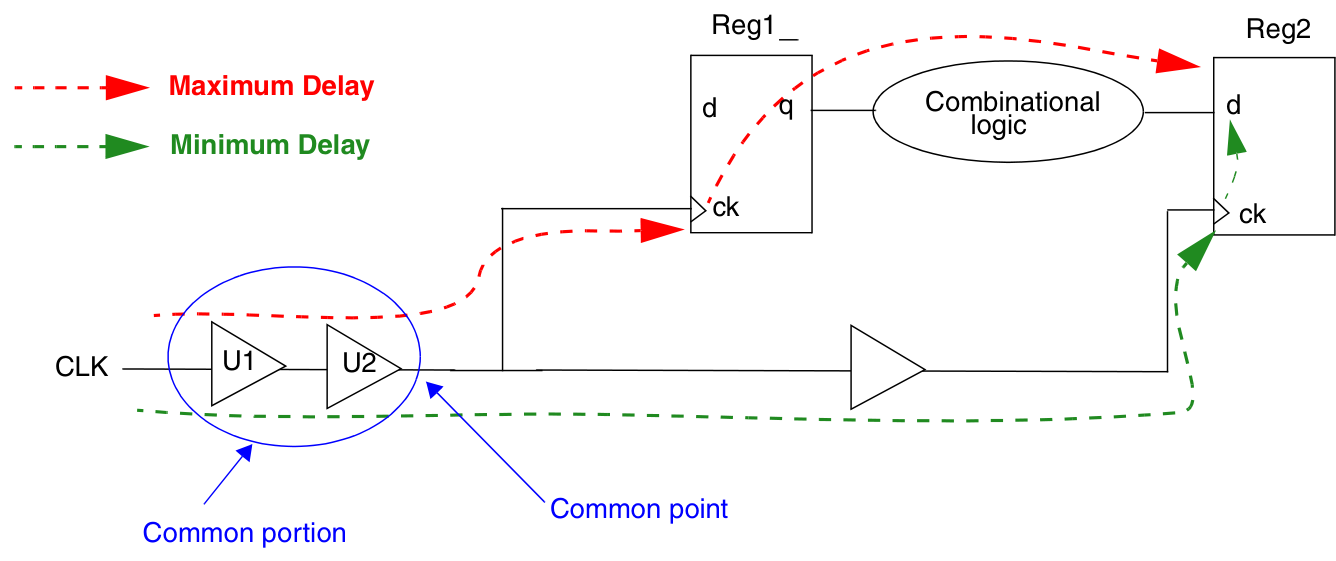
\includegraphics[width=0.9\textwidth]{fig-4-4.png}
  \caption{时钟再汇聚悲观量示例}
  \label{fig:crp}
\end{figure}

setup 分析时，对公共部分，工具对 launch 路径使用最大延迟、对 capture 路径使用最小延迟，从而产生时钟再汇聚悲观量。

从时钟源扇出到时序器件数据引脚、且 launch 与 capture 路径共享一段时钟路径的路径上，也可能引入悲观量，如图~\ref{fig:crp-fanout}。

\begin{figure}[htbp]
  \centering
  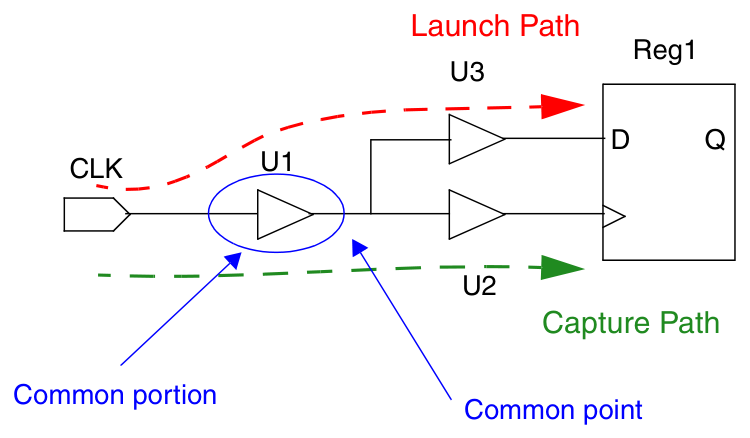
\includegraphics[width=0.72\textwidth]{fig-4-5.png}
  \caption{从时钟源扇出到数据引脚的时序路径}
  \label{fig:crp-fanout}
\end{figure}

\section{启用时钟再汇聚悲观量消除}
\subsection*{Enabling Clock Reconvergence Pessimism Removal}

把应用选项 \appopt{time.remove\_clock\_reconvergence\_pessimism} 设为 \cmd{true} 以启用 CRPR。默认值为 \cmd{false}，不执行 CRPR。

启用 CRPR 会使分析更不悲观，但会增加运行时间与内存占用。该变量的任何改变都会引起一次完整的时序更新。

还可以用下列应用选项进一步控制 CRPR：
\begin{itemize}
  \item 用 \appopt{time.clock\_reconvergence\_pessimism} 决定对公共部分上同极性或反极性的时钟跳变是否消除悲观量：
  \begin{itemize}
    \item \cmd{same\_transition}：仅当公共部分中的时钟跳变极性相同时才做 CRPR。
    \item \cmd{normal}：对公共部分中同极性与反极性的时钟跳变都做 CRPR。这是默认值。
  \end{itemize}
  \item 把 \appopt{time.crpr\_remove\_clock\_to\_data\_crp} 设为 \cmd{true}，消除 clock-to-data 路径与时钟路径之间的悲观量。默认值为 \cmd{false}。
\end{itemize}

\section{报告时钟再汇聚悲观量消除的计算}
\subsection*{Reporting Clock Reconvergence Pessimism Removal Calculations}

\cmd{report\_crpr} 报告两个寄存器时钟引脚或端口之间的 CRP 计算。需要指定 launch 与 capture 寄存器的引脚、时钟，以及检查类型（setup 或 hold）。例如：
\begin{lstlisting}
icc2_shell> report_crpr -from [get_pins ffa/CP] \
    -to [get_pins ffd/CP] -setup
\end{lstlisting}

该命令生成的报告给出：
\begin{itemize}
  \item 公共点的位置
  \item launch 与 capture 时钟边沿类型（上升或下降）
  \item 公共点处四个计算得到的到达时间（early 与 late，以及 rise 与 fall）
  \item 计算得到的 CRP 值（rise 与 fall）
  \item 用于 opening-edge 与 closing-edge 悲观量消除的值
\end{itemize}

\cmd{report\_crpr} 报告的 CRP 量可能与 \cmd{report\_timing} 略有不同。为提高计算效率，当相邻点之间的 CRP 差异过小时，\cmd{report\_timing} 会把多个点合并后再做 CRPR 计算。
